\providecommand{\main}{../}
\documentclass[../writeup.tex]{subfiles}

\begin{document}  


\section{Methods}


\subsection{Joint Demultiplex and Upsample}

One approach which we can consider involves the following steps
\begin{enumerate}
    \item Use $\widetilde{\bC}$ for bucket activities and capture the two-bucket image $\bY$
    \item Recover full resolution images $\bX$ under $S$ illuminations from $\bY$ by solving a linear inverse problem
    \item use $\bX$ to solve for phase and albedo using ZNCC decoding \cite{mirdehghanOptimalStructuredLight2018}
\end{enumerate}
Instead of treating upsampling (recover $2F$ images $\sI$ from $2$ images $\bY$) and demultiplexing (recover $S$ images $\bX$ from $2F$ images $\sI$) as distinct steps, we aim to recover $\bX$ directy from $\bY$, in a single step, by solving a linear inverse problem. Jointly upsample and demultiplex enforces a prior knowledge of image formation and reduces accumulation of error at each image processing step \cite{heideFlexISPFlexibleCamera2014}. This approach allows encoding arbitrary subsampling schemes in the forward operator and can be adapted to any frames $F$. 

\paragraph{MAP Inference with Implicit Regularizer}
Assuming an isotropic Gaussian noise model ($\by=\bA\bx + \be$ where $\be\sim \sN(0,\sigma^2 \bI)$), and prior $p_{\rx}(x) \propto \exp\pc{- (\lambda/\sigma^2) \Gamma(\bx) }$ where $\Gamma:\R^{SP}\to\R$ is some regularizer for $\bx$. Given noisy measurement $\by$, \textit{max a posterior} estimate $\hat{\bx}$ can be obtained by solving the following
\begin{align}
    \text{minimize}_{\bx}\;\;
        \frac{1}{2} \norm{\bA\bx-\by}_2^2 + \lambda \Gamma(\bx)
    \label{eq:generic_prior_inverse_problem}
\end{align}
where $\lambda$ is weight for the regularizer. 

\paragraph{Optimization Using PnP/RED}
We solve (\ref{eq:generic_prior_inverse_problem}) using PnP/RED \cite{venkatakrishnanPlugandPlayPriorsModel2013,romanoLittleEngineThat2016}, which use denoisers in place of a proximal operator under a ADMM style updates. We can specialize the update equations to our problem. First we notice that $\bA\bA^T$ is diagonal when $\bW$ is the optimal bucket multiplexing matrix constructed from Hadamard matrix specified in \cite{weiCodedTwoBucketCameras2018}. The x-update can be simplified  \cite{liuRankMinimizationSnapshot2019} 
\begin{align}
    \bx^{k+1} 
        = \tilde{\bx} + \bA^T \begin{bmatrix}
            \frac{(\by - \bA\tilde{x})_1}{\bzeta_1 + \rho},\cdots, \frac{(\by - \bA\tilde{\bx})_{SP}}{\bzeta_{SP} + \rho}
        \end{bmatrix}^T
    \label{eq:red_x_desci_update}
\end{align}
where $\rho$ is the parameter for augmented lagrangian, $\tilde{\bx} = \bz^k - \bu^k$, and $\bzeta = \diag \left(\bA\bA^T\right)$, which can be precomputed. (\ref{eq:red_x_desci_update}) is fast because it consists of 2 sparse matix-vector multiply and a few element-wise vector operations. The update equations is then
\begin{align} 
    \bx^{k+1}
        &= \tilde{\bx} + \bA^T \begin{bmatrix}
            \frac{(\by - \bA\tilde{x})_1}{\bzeta_1 + \rho},\cdots, \frac{(\by - \bA\tilde{\bx})_{SP}}{\bzeta_{SP} + \rho}
        \end{bmatrix}^T
        \qquad \tilde{\bx} = \bz^k - \bu^k \\
    \bz^{k+1}
        &= \frac{1}{\rho + \lambda} \left(
            \lambda \sD(\bz^{k}) + \rho ( \bx^{k+1} + \bu^k  )
        \right) \\
    \bu^{k+1}
        &= \bu^k + \bx^{k+1} - \bz^{k+1}
    \label{eq:red_admm_update_equations_fast_x_update}
\end{align}
Note this method is general enough to allow for both multispectral imaging, structured light reconstruction, and perhaps a mix of the two modalities.

 

\subsection{Correspondence Refinement}
In applications where we are purely interested in structured light reconstruction. There are artifacts associated with spatial subsampling when number of illuminated patterns gets larger. Here we exploit a simple image formation model under active illumination to refine correspondence.


\begin{figure}[h!]
    \begin{center}
        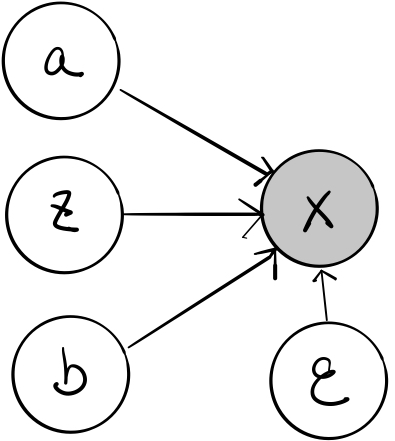
\includegraphics[height=3cm]{draw_phase_signal_image_formation_model}
        \caption{Reconstructed Images $\bX$ and its relationship to albedo, phase, and ambient illumination.}
        \label{fig:draw_phase_signal_image_formation_model}
    \end{center}
\end{figure}  

\paragraph{Image Formation Under Active Illumination}

Let $\ba \in \R_+^{P}$ be albedo, $\bb\in\R_+^P$ be ambient illumination, $\bz\in[0,1]^{P}$ be correspondence/phase. We consider the following probabilistic model as depicted in Figure~\ref{fig:draw_phase_signal_image_formation_model}. In particular, we assume Gaussian noise $\bepsilon\in\sN(0,\sigma^2_{\epsilon}\bI)$ capturing errors in model misspecification, then we have per-pixel image formation model
\begin{align}
    \si^p
        &= \ba^p \bl(\bz^p) + \bb^p + \bepsilon^p
        \qquad
        p = 1,2,\cdots,P
    \label{eq:per_pixel_image_formation_patterned_image}
\end{align}
where $\bl:[0,1]\to [0,1]^S$ where $\bl(z) = (\bl_1(z),\cdots,\bl_S(z))$ is vector valued function that specifies illumination condition at a particular projector index $z$, normalized to lie in $[0,1]$. From perspective of structured light coding, $\bl$ is the coding scheme for the system. It might be interesting to extend (\ref{eq:per_pixel_image_formation_patterned_image}) to include effect of global illumination and defocus, similar to \cite{guptaMicroPhaseShifting2012}. Note the relationship in (\ref{eq:per_pixel_image_formation_patterned_image}) is nonlinear and nonconvex, due to coupling of albedo and illumination conditions. Given $\bz$, the relationship becomes linear
\begin{align}
    \vec{\bX^T}
        =
    \begin{bmatrix}
        \si^1 \\
        \vdots \\
        \si^P \\
    \end{bmatrix}
        =
        \underbrace{
            \begin{bmatrix}
                \diag \bl(\bz^1) & \bI \\ 
                \vdots & \vdots \\ 
                \diag \bl(\bz^P) & \bI \\
            \end{bmatrix}
        }_{\bM(\bz)}
        \begin{bmatrix}
            \ba \\ \bb 
        \end{bmatrix}
    \label{eq:per_pixel_image_formation_patterned_image_given_correspondence}
\end{align}


\paragraph{MAP Inference of Correspondence}

For arbitrary patterns, the MAP estimate of a discrete set of correspondences is very hard, as it involves a combinatorial problem over a very high dimensional space, in particular $L^P$ possible combinations. For convenience of optimization, we assume $\bl$ be a coordinate-wise continuous function, and we are interested in finding correspondence in the real numbers. A similar bayesian setup for solving depth and albedo is detailed in \cite{adamBayesianTimeofFlightRealtime2015}. Assuming uniform prior for $\ba,\bb$, we have
\begin{align}
    \hat{\ba},\hat{\bb},\hat{\bz}
        = \argmax_{a,b,z} p_{\ra,\rb,\rz|\rx}(a,b,z|x)
        = \argmin_{a,b,z} -\log p_{\rx|\ra,\rb,\rz}(x|a,b,z) - \log p_{\rz}(z)
    \label{eq:map_inference_of_correspondence_is_hard}
\end{align}
Assumption of Gaussian noise in (\ref{eq:per_pixel_image_formation_patterned_image}) and $p_{\rz}(z)\propto \exp\pc{ - (\lambda/\sigma_{\epsilon}^2) \norm{\bG \bz}_1 }$ ($\bG=[\bG_x;\bG_y]\in \R^{2P\times P}$ are the differencing matrix for computing total variation norm) yield the following optimization problem
\begin{align}
    \underset{ \ba\in\R_+^P,\bb\in\R_+^P,\bz\in [0,1]^P }{\text{minimize}}\;\;
        \frac{1}{2} \sum_{ p=1 }^P \norm{ \si^p - \ba^p \bl(\bz^p) - \bb^p }_2^2 + \lambda \norm{\bG \bz}_1
    \label{eq:tv_regularized_ls_for_solving_correspondence}
\end{align}
Without assumption of coordinate-wise convexity of $\bl$, the objective function is subject to bad local minimas. Idea is to seed the nonlinear optimization procedure with ZNCC decoding of $\bx$ solved by (\ref{eq:red_admm_update_equations_fast_x_update}) and hope that this refinement will get us to the destination. To make optimization easier (\ref{eq:tv_regularized_ls_for_solving_correspondence}), similar to \cite{rosmanSparseModelingShape2012}, we use block coordinate descent to optimize for $\ba,\bb$ and $\bz$ in an alternating fashion,
\begin{align}
    \ba_{k+1},\bb_{k+1}
        &= \argmin_{\ba\in\R_+^P,\bb\in\R_+^P} \norm{ \bM(\bz_k) \begin{bmatrix}
            \ba \\ \bb
        \end{bmatrix} - \vec{\bX^T} }_2^2 
    \label{eq:tv_regularized_ls_for_solving_correspondence_altmin_1} \\
    \bz_{k+1}
        &= \argmin_{\bz\in[0,1]^P} \frac{1}{2} \sum_{ p=1 }^P \norm{ \si^p - \ba_{k+1}^p \bl(\bz^p) - \bb_{k+1}^p }_2^2 + \lambda \norm{\bG \bz}_1 
    \label{eq:tv_regularized_ls_for_solving_correspondence_altmin_2}
\end{align}
where (\ref{eq:tv_regularized_ls_for_solving_correspondence_altmin_1}) can be solved with any sparse linear solver, and (\ref{eq:tv_regularized_ls_for_solving_correspondence_altmin_2}) can be solved using some nonlinear solver such as lbfgs as it emits computable sub-gradients 
\begin{align}
     -\sum_{s=1}^S 
            \left( \si^p - \ba^p \bl_s(\bz^p) - \bb^p \right) \ba^p g_s(\bz^p)
            + \lambda \left( \bG^T \textsf{sgn}\left( \bG \bz \right) \right)_p
        \in \partial_{\bz^p}(\cdot)
    \label{eq:tv_regularized_ls_for_solving_correspondence_altmin_1_gradient}
\end{align}
where $g_s(\bz^p) \in \partial_{z}\bl_s(\bz^p)$. In case when $\bl$ is coordinate-wise convex, the objective for (\ref{eq:tv_regularized_ls_for_solving_correspondence}) is a bi-convex problem, which enjoys certain conergence properties. Optimizing multi-convex function has been explored in applications such as time-of-flight reconstruction \cite{heideNonlineofsightImagingPartial2017}. 

\paragraph{Applicable Coding Schemes}

Empirically, the choice of $\bl$ is very important for optimization. Some coding schemes are more well behaved, for example spatial sinusoids with frequency of 1 shifted multiple times. Spatial sinusoids with spatial frequency $> 2$, micro phase shifting code \cite{guptaMicroPhaseShifting2012}, Hamiltonian code \cite{guptaGeometricPerspectiveStructured2018}, a la carte code \cite{mirdehghanOptimalStructuredLight2018} all give rise to objective functions in (\ref{eq:tv_regularized_ls_for_solving_correspondence}) with bad local minima. One potential way to alleviate this is perhaps to design coding schemes that are coordinate-wise convex, which will ensure that the objective function is bi-convex.


\subsection{Revised Noise Model}
We might argue the Gaussian model assumption does actually reflect the physical reality. In particular, sensor noise happens when the images $\bY$ are acquired, as depicted in Figure~\ref{fig:draw_phase_c2b_image_formation_model}.


\begin{figure}[h!]
    \begin{center}
        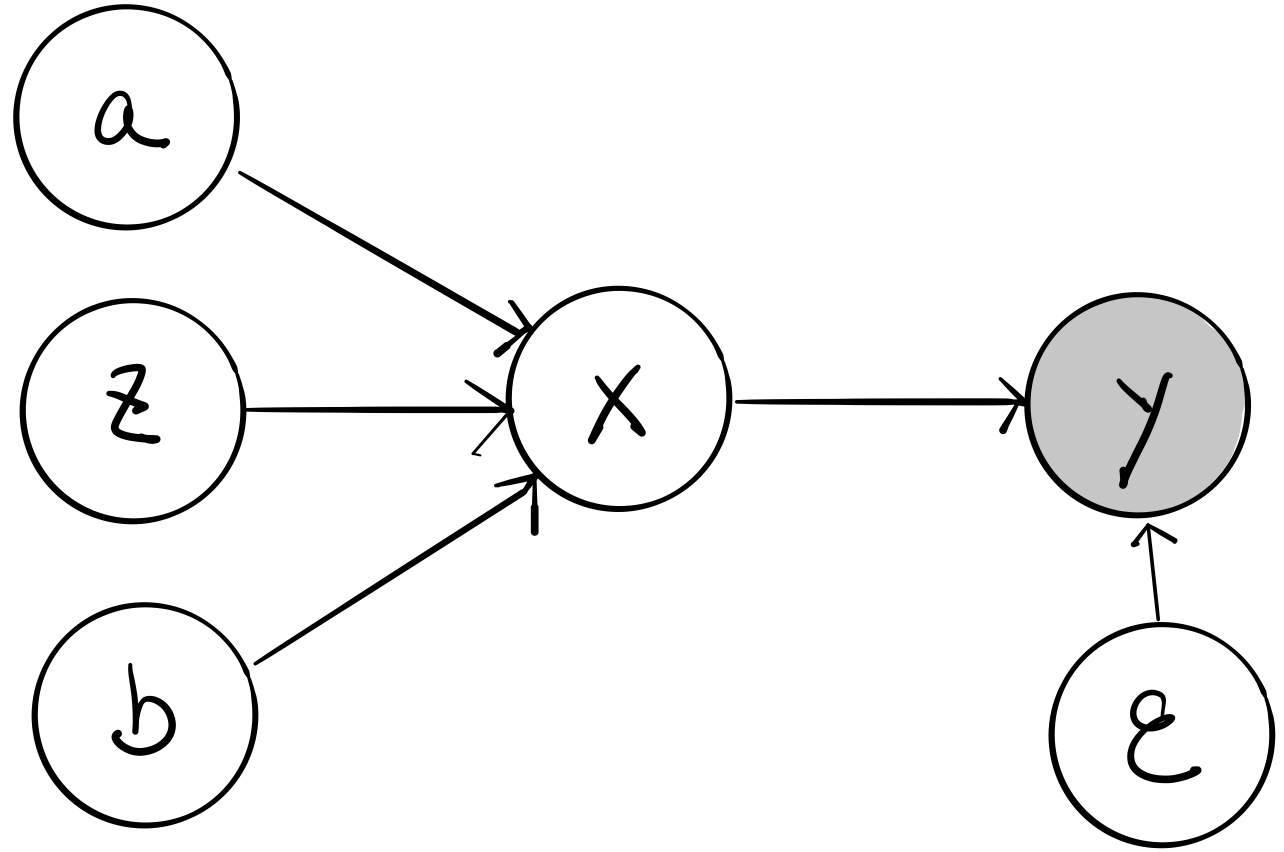
\includegraphics[height=3cm]{draw_phase_c2b_image_formation_model}
        \caption{c2b measurements $\bY$ and its relationship to albedo, phase, and ambient illumination}
        \label{fig:draw_phase_c2b_image_formation_model}
    \end{center}
\end{figure}  






\subsection{Experimental Results}

\paragraph{Ground Truth} Ground truth phase/disparity is obtained by computing ZNCC decoding on sinusoids of periods 1,2,5,17,31, each shifted 30 times. Each measurement under a unique illumination pattern is stacked form 250 noisy images. 

\paragraph{Empirical Performance Upper Bound} In Figure~\ref{fig:sinusiods_spatial_freq_1_phase_upper_bound_wrt_S}, we experimentally determine what is empirically possible for the decoding algorithm, without either noise nor recosntruction error, when given measurement under different number of phase shifts, assuming sinusoidal pattern with period 1.
\begin{figure}[h!]
    \begin{center}
        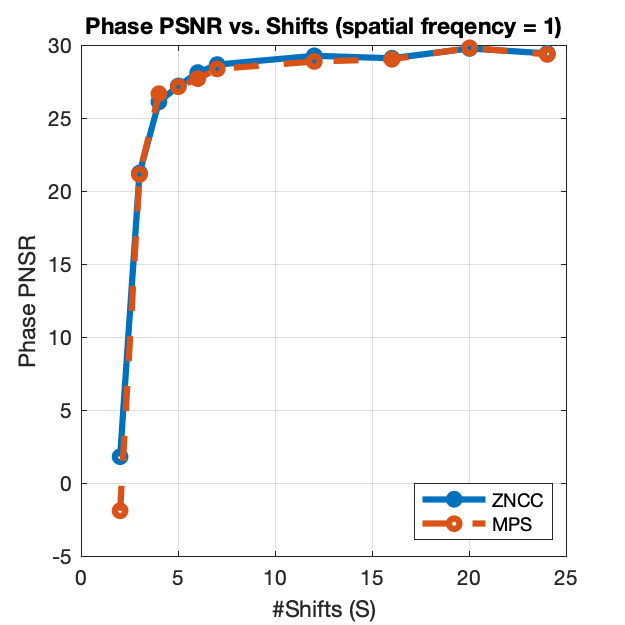
\includegraphics[width=0.49\textwidth]{SinusoidsSpatialFreq1PhaseUpperBoundPSNR}
        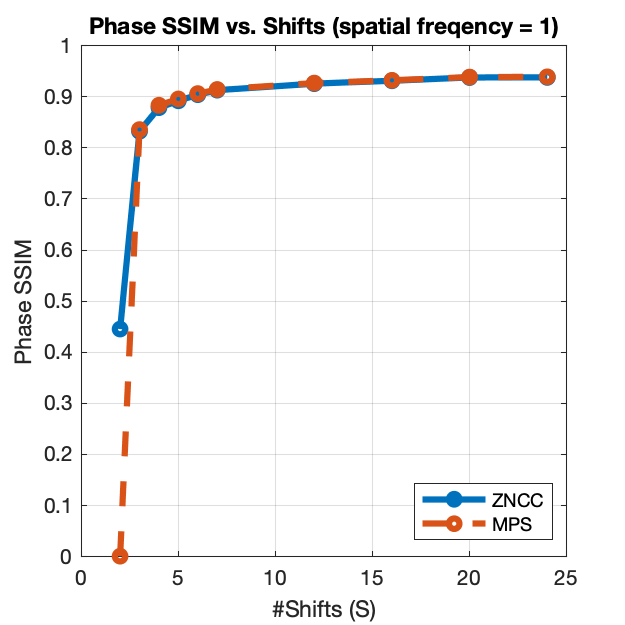
\includegraphics[width=0.49\textwidth]{SinusoidsSpatialFreq1PhaseUpperBoundSSIM}
        \caption{PSNR/SSIM computed by comparing phase obtained by ZNCC/MPS decoding on stacked noiseless images for sinusoidal pattern with period of 1 with varying number of phase shifts to the ground-truth phase. Both decoder performed similarly. We see large improvement when $S=3,4$ and minimal improvement when $S>7$.}
        \label{fig:sinusiods_spatial_freq_1_phase_upper_bound_wrt_S}
    \end{center}
\end{figure}  


% \newpage\newpage
% \subsection{Solving Inverse Problem using RED}

% We first note that the illumination ratios are albedo quasi-invariant, and therefore smooth within object boundaries. Therefore, total variation regularization on illuination ratio images could be particularly effective. To avoid extra notations, we use $\bx,\by$ as the corresponding illumination ratios that we want to reconstruct. Additionally, we adapt algorithm in \cite{romanoLittleEngineThat2016} for imposing algorithm induced priors with state-of-the-art denoisers. In summary, we want to optimize the following constrained problem with a set of affine constraints,
% \begin{align*}
%     \minimize  & \norm{\bA\bx_1 - \by}_2^2 + \frac{\lambda_2}{2} \bx_2^T(\bx_2 - \sD(\bx_2)) + \lambda_3 \norm{\bx_3}_1 \\
%     \subjectto & \bx_1 - \bx_2 = 0 \\
%                & \bG\bx_1 - \bx_3 = 0 \\
% \end{align*}
% where $\bx_1,\bx_2\in\R^{SP}$, $\bx_3\in\R^{2SP}$. $\lambda_2,\lambda_3>0$ are weights to the regularizers. $\bG\in \R^{2SP\times SP}$ is the discrete image gradient for $S$ images 
% \[
%     \bG =
%     \begin{bmatrix}
%         \bI_S \otimes \bG_x \\
%         \bI_S \otimes \bG_y \\
%     \end{bmatrix} 
% \]
% where $\bG_x,\bG_y\in\R^{P\times P}$ are the discrete image gradients for a single image computed using forward difference. We can gather constraints into a single linear system 
% \[
%     \bH\bx = 0
%     \quad\quad \text{where}\quad\quad
%     \bH = 
%     \begin{bmatrix}
%         \bI_{SP} & -\bI_{SP} & 0  \\
%         \bG    & 0    & -\bI_{SP}  \\
%     \end{bmatrix}
%     \quad
%     \bx = 
%     \begin{bmatrix}
%         \bx_1 \\ \bx_2 \\ \bx_3
%     \end{bmatrix}
% \]
% and arrive at an equivalent optimization problem
% \begin{equation}
%     \label{eq:method_optimization_problem}
%     \begin{aligned}
%         \minimize  & f_1(\bx_1) + \lambda_2 f_2(\bx_2) + \lambda_3 f_3(\bx_3) \\
%         \subjectto & (\bx_1,\bx_2,\bx_3) \in \sC
%     \end{aligned}
% \end{equation}
% where $\sC = \{\bx\in\R^{4SP} \;\mid\; \bH\bx = 0\}$ and 
% \begin{align*}
%     f_1(\bx_1)
%         &=\norm{\bA\bx_1 - \by}_2^2 \\
%     f_2(\bx_2)
%         &=\frac{1}{2} \bx_2^T(\bx_2 - \sD(\bx_2)) \\
%     f_3(\bx_3)
%         &=\norm{\bx_3}_1
% \end{align*}

% \subsection{Optimization}

% As shown below, the scaled form ADMM for solving (\ref{eq:method_optimization_problem}) is given by 
% \begin{align*}
%     \bx_1^{k+1}
%         &= \prox_{(1/\rho)f_1}(\bz_1^k - \bu_1^k) 
%         = (I + \frac{2}{\rho} A^TA)^{-1} ( \bz_1^k - \bu_1^k + \frac{2}{\rho}A^T y) \\
%     \bx_2^{k+1}
%         &= \prox_{(\lambda_2/\rho)f_2}(\bz_2^k - \bu_2^k) 
%         = \frac{1}{\lambda_2+\rho} (\lambda_2 \sD(\bx_2^k) + \rho(\bz_2^k - \bu_2^k)) \\
%     \bx_3^{k+1}
%         &= \prox_{(\lambda_3/\rho)f_3} (\bz_3^k - \bu_3^k) 
%         = \sS_{\lambda_3/\rho}(\bz_3^k - \bu_3^k) \\
%     \bz^{k+1}
%         &= \prox_{(1/\rho)\sI_{\sC}}(\bx^{k+1} + \bu^k)
%         = (I - \bH^{\dagger}\bH)(\bx^{k+1}+\bu^k) \\
%     \bu^{k+1}
%         &= \bu^{k} + \bx^{k+1} - \bz^{k+1}
% \end{align*}



\end{document}

